\documentclass[]{../template/Report}%方括号内写yuxi即生成预习报告\documentclass[yuxi]{../template/Report}
\settemplatedir{../template/}%设置模板路径
\usepackage{enumitem}
\exname{金属材料杨氏模量的测定} %实验名称
\extable{} %实验桌号
\instructor{} %指导教师
\class{} %班级
\name{} %姓名
\stuid{} %学号

\nyear{} %年
\nmonth{} %月
\nday{} %日
\nweekday{} %星期几,e.g. \nweekday{三}
\daypart{}%上午/下午

\redate{} %如有实验补做,补做日期
\resitu{} %情况说明:

\begin{document}
\maketitle%输出封面

\section{预习报告(10分)}
\subsection{实验综述(5分)}
\subsubsection{实验原理}
\paragraph{杨氏模量}
对于长度为$L$、横截面积为$S$的均匀金属丝,在其两端施加外力$F$时,金属丝单位面积上所受的力$F/S$称为正应力,相应的相对伸长量$\Delta L/L$称为线应变。根据胡克定律,在弹性限度内,应力与应变成正比,其比例系数定义为杨氏模量$E$,表达式为:
\begin{equation}
E = \frac{FL}{S\Delta L}
\end{equation}
杨氏模量是表征材料抵抗弹性形变能力的物理量,其值越大,材料的刚性越强,越难发生弹性形变。

\paragraph{光杠杆法测量原理}
由于金属丝的伸长量$\Delta L$十分微小,直接测量困难,本实验采用光杠杆法进行间接测量。光杠杆装置由一个带有三足的平面镜构成,三足尖构成等腰三角形,其后足到前两足连线的垂直距离记为$b$。

测量时,标尺经平面镜反射后在望远镜中成像。初始状态下,望远镜十字叉丝对应的标尺读数为$S_0$。当金属丝在外力作用下伸长$\Delta L$时,光杠杆后足随之下降,使平面镜绕前两足连线转过$\theta$角,此时望远镜中的标尺读数变为$S_1$。

根据几何光学原理,反射光线的偏转角为$2\theta$,当$\theta$很小时,有:
\begin{equation}
\tan 2\theta \approx 2\theta = \frac{\Delta S}{D}, \quad \tan \theta \approx \theta = \frac{\Delta L}{b}
\end{equation}
其中$\Delta S = S_1 - S_0$,$D$为镜面到标尺的垂直距离。由上两式可得:
\begin{equation}
\Delta S = \frac{2D}{b}\Delta L
\end{equation}
这表明标尺读数的变化量$\Delta S$是实际伸长量$\Delta L$的$2D/b$倍,该比值称为光杠杆的放大倍数。

将金属丝的横截面积$S = \pi d^2/4$($d$为直径)代入杨氏模量定义式,整理得:
\begin{equation}
E = \frac{8FLD}{\pi d^2 b \Delta S}
\end{equation}

\subsubsection{实验方法}
\paragraph{系统调节}
\begin{itemize}
\item 调节底座螺丝使立柱处于铅直状态,预先施加2kg负荷使金属丝伸直
\item 正确放置光杠杆,确保平面反射镜镜面铅直
\item 将望远镜置于距光杠杆约1.5m处,调节其高度和方位,使望远镜光轴与镜面中心等高,最终在望远镜中看到清晰的标尺像
\end{itemize}

\paragraph{伸长量测量}
\begin{itemize}
\item 首先读取初始负荷(2kg)下的标尺读数$S_0$
\item 依次增加1kg砝码,分别记录相应的标尺读数$S_1, S_2, \cdots, S_7$
\item 再依次减少1kg砝码,记录对应的读数$S_7', S_6', \cdots, S_0'$
\item 采用逐差法处理数据,计算伸长量$\Delta S$
\end{itemize}

\paragraph{参数测量}
\begin{itemize}
\item $b$的测量:将光杠杆三足压印在白纸上,作前两足连线,用游标卡尺测量后足到该连线的垂直距离
\item $L$的测量:用钢卷尺测量金属丝上下夹头间的有效长度
\item $d$的测量:用螺旋测微计在金属丝不同位置多次测量直径
\item $D$的测量:用卷尺测量标尺到镜面的垂直距离
\end{itemize}

\paragraph{数据处理}
根据测量数据计算杨氏模量$E$的值,并用不确定度理论评估测量结果的可靠性。

\subsection{实验重点}
\begin{enumerate}
\item 掌握杨氏模量的物理意义及拉伸法测量原理
\item 理解光杠杆放大原理,熟练掌握光路调节技术
\item 学会用逐差法处理数据,掌握不确定度的计算方法
\end{enumerate}

\subsection{实验难点}
本实验的主要操作难点体现在以下几个方面:

\begin{enumerate}
\item \textbf{系统初始状态调节}:需确保杨氏模量仪底座严格水平、双立柱铅直,这对后续测量的准确性至关重要。同时,需要通过上下夹具牢固固定金属丝,保证其在拉伸过程中保持严格的竖直状态,避免与平台孔壁接触产生摩擦。

\item \textbf{光路系统精细调节}:此为本实验的核心难点。需要同时满足多个光学条件:平面反射镜镜面严格铅直;望远镜光轴与反射镜共轴;消除视差使标尺像与叉丝在同一平面。此过程需要耐心和技巧,对观察能力和细致程度要求较高。

\item \textbf{测量过程中的稳定性控制}:手动逐级加减砝码时,需保持动作平稳轻柔,避免引起金属丝和光杠杆系统的晃动。任何突然的冲击都可能导致光杠杆足尖移位或金属丝异常振动,从而引入显著的随机误差。

\item \textbf{异常情况的诊断与处理}:当望远镜中无法找到标尺像时,需要从镜筒外目视辅助判断光路,并系统性地调整望远镜方位或镜面角度。当读数出现异常波动时,需要能够准确判断是由于夹头松动、装置未调垂直、还是超出弹性限度等原因所致。
\end{enumerate}
\begin{fullreportonly}
\section{原始数据(20分)}
(将有老师签名的“自备数据记录草稿纸”的扫描或手机拍摄图粘贴在下方,完整保留姓名,学号,教师签字和日期。)
\begin{figure}[H]
    \centering
    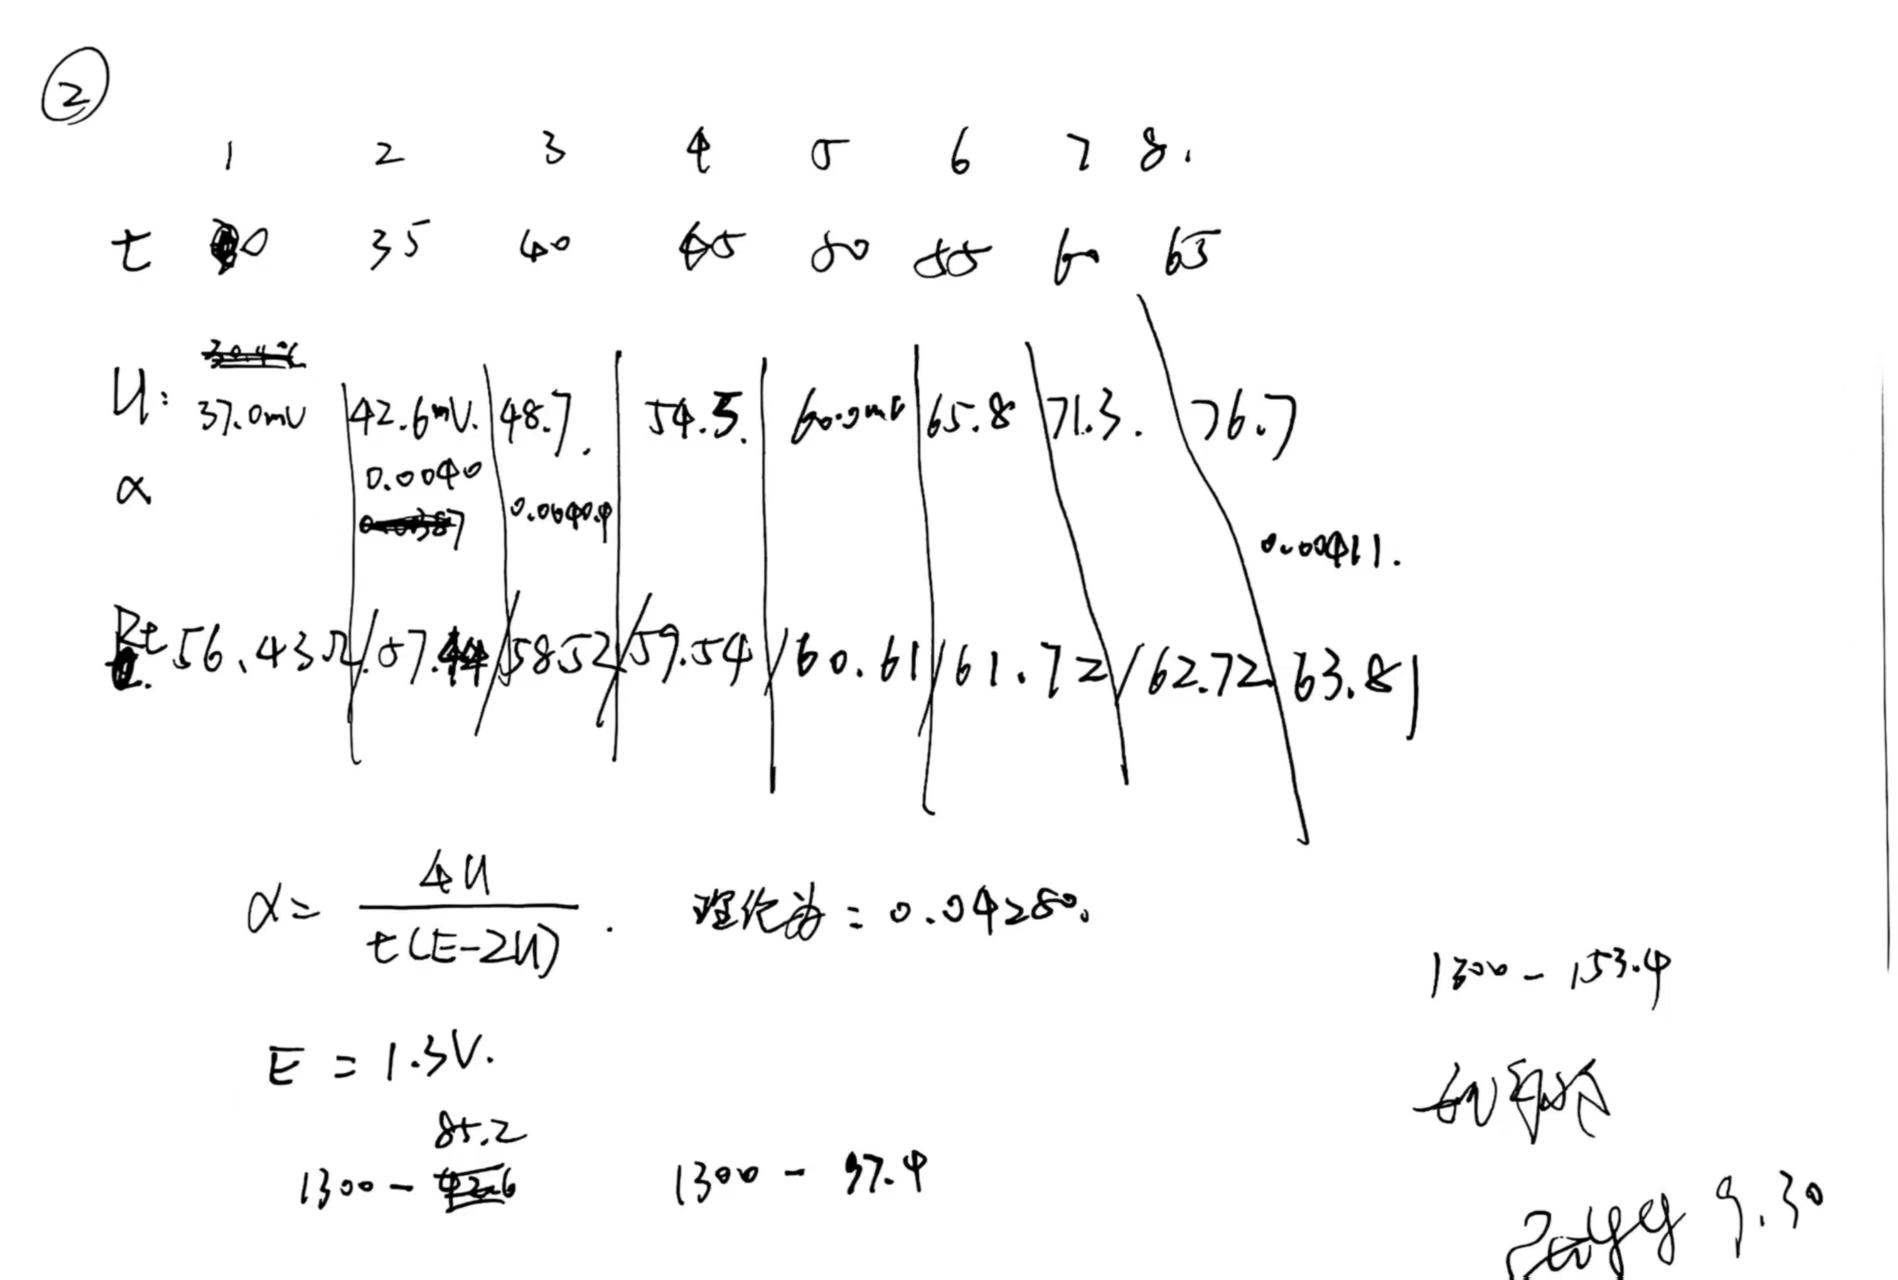
\includegraphics[width=0.6\textwidth]{原始数据.jpg}
    \caption{原始数据记录}
    \label{fig:原始数据记录}
\end{figure}
\section{结果与分析(60分)}
\subsection{数据处理与结果(30分)}
(列出数据表格、选择适合的数据处理方法、写出测量或计算结果。)
\subsubsection{$\Delta S$测量结果及处理}
	\begin{table}[H]
		\centering
		\label{tab:exp_data}
		\begin{tabular}{|c|c|c|c|c|}
			\hline
			\textbf{次数} & \textbf{作用力$F=mg$/(kg)} & \textbf{加砝码读数/(cm)} & \textbf{减砝码读数/(cm)} & \textbf{平均值/(cm)} \\
			\hline
			1 & 1 & -11.61 & -11.35 & -11.48 \\
			\hline
			2 & 2 & -10.79 & -10.65 & -10.72 \\
			\hline
			3 & 3 & -10.12 & -9.93 & -10.03 \\
			\hline
			4 & 4 & -9.30 & -9.15 & -9.23 \\
			\hline
			5 & 5 & -8.58 & -8.52 & -8.55 \\
			\hline
			6 & 6 & -7.88 & -7.79 & -7.84 \\
			\hline
			7 & 7 & -7.12 & -7.08 & -7.10 \\
			\hline
			8 & 8 & -6.37 & -6.30 & -6.34 \\
			\hline
		\end{tabular}
	\end{table}
\subsubsection{D,b,L,d测量结果及处理}
	\begin{table}[H]
		\centering
		\label{tab:exp_data}
		\begin{tabular}{|c|c|c|c|c|}
			\hline
			\textbf{次数} & \textbf{D/(cm)} & \textbf{b/(cm)} & \textbf{L/(cm)} & \textbf{d/(cm)} \\
			\hline
			1 & 141.35 & 73.66 & 115.32 & 0.623 \\
			\hline
			2 & 141.44 & 73.74 & 115.43 & 0.623 \\
			\hline
			3 & 141.39 & 73.89 & 115.43 & 0.621 \\
			\hline
			4 & 141.41 & 73.86 & 115.47 & 0.625 \\
			\hline
			5 & 141.34 & 72.80 & 115.49 & 0.625 \\
			\hline
			6 & 141.52 & 73.81 & 115.45 & 0.624 \\
			\hline
			平均值 & 141.41 & 73.79 & 115.43 & 0.624 \\
			\hline
		\end{tabular}
	\end{table}

\subsubsection{杨氏模量的计算}
\paragraph{直接计算法}
\begin{equation}
E=\frac{8FLD}{\pi d^2 b \Delta S}=1.95E+11 Pa
\end{equation}
\begin{equation}
\frac{u(E)}{E}=\sqrt{(\frac{u(F)}{F})^2+(\frac{u(L)}{L})^2+(\frac{u(D)}{D})^2+(\frac{2u(d)}{d})^2+(\frac{u(b)}{b})^2+(\frac{u(\Delta S)}{\Delta S})^2}=3.30E-04
\end{equation}
\begin{equation}
\Rightarrow  u(E)=6.43E+07 Pa
\Rightarrow E=(1.9500\pm0.0006)E+11 Pa
\end{equation}
\paragraph{作图法}
作出$\Delta S-F曲线图$,如图\ref{fig:图表法}所示,利用线性拟合得到斜率k=0.7305cm/kg,由$\frac{1}{K}=\frac{\pi d^2 b}{8DL}E$知,E=1.95E+11 Pa。
\begin{figure}[H]
    \centering
    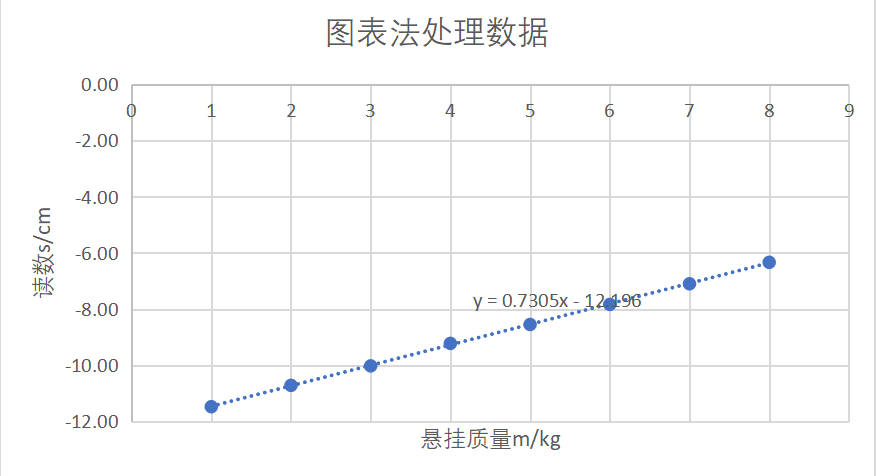
\includegraphics[width=0.6\textwidth]{图表法.jpg}
    \caption{图表法}
    \label{fig:图表法}
\end{figure}
\subsection{误差分析(20分)}
\begin{enumerate}
\item \textbf{长度测量的系统误差与人为误差:} 实验涉及钢丝长度$L$、光杠杆镜臂长$b$、镜尺距离$D$及钢丝直径$d$等多个长度量的测量。其中,$b$、$D$、$L$使用米尺测量,估读位存在主观性;而直径$d$需用螺旋测微计在钢丝不同位置多次测量,若夹持过紧或位置分布不均,会引入误差。这些长度量的不确定度将共同影响杨氏模量$E$的最终结果。
\item \textbf{外力$F$的标定误差:} 实验中默认每个砝码质量为1.000kg,但实际质量与标称值存在偏差。若直接使用标称值计算力$F$的变化,会系统性地偏离真实的$\Delta S-F$关系。为减小此误差,可精确测定每个砝码的实际质量,并用以绘制更准确的$\Delta S-F$关系图。
\item \textbf{形变量$\Delta S$的动态读数误差:} 加减砝码后,钢丝与支架系统需经历一段阻尼振动才能静止。若未待系统稳定即进行读数,或因环境扰动(如风吹、走动)导致光杠杆镜或望远镜微小振动,会使标尺刻度$S$在平衡位置附近波动,给$\Delta S$的测量带来随机误差。
\item \textbf{光路与仪器调节不完善带来的误差:} 这是影响$\Delta S$测量准确性的关键。若实验初光杠杆镜面未严格铅直、望远镜光轴未水平或未能清晰消视差,将导致标尺像歪斜、模糊或存在视差。此状态下测得的$\Delta S$会系统性偏离理论值$\frac{2D}{b}\Delta L$,且该误差难以在后续数据处理中消除。
\end{enumerate}
\subsection{实验难点(2分)}
\begin{enumerate}
\item \textbf{系统调节:} 确保杨氏模量仪支柱垂直,避免金属丝夹头与平台孔壁摩擦;通过上下夹具紧固金属丝,保证拉伸方向严格沿竖直方向。
\item \textbf{光杠杆调节:} 需准确调节反射镜面竖直,并使望远镜与光杠杆共轴、对焦清晰以消除视差。
\item \textbf{砝码操作:} 需平稳地逐级加减砝码,避免因操作晃动引起光杠杆足尖移动或金属丝异常伸缩。
\item \textbf{成像与读数:} 初调时若望远镜中看不到标尺像,需从镜筒外目视判断并调整镜面角度或望远镜位置;若叉丝不清,调节目镜焦距。读数不稳定可能源于夹头松动、金属丝超弹性范围或装置不垂直等因素。
\end{enumerate}
\subsection{实验探讨(10分)}
本实验采用拉伸法法结合光杠杆仪器测量金属丝的杨氏模量。关键在于光路系统的精细调节与稳定,以及在弹性限度内通过逐次加载、卸载砝码获取形变数据。实验表明,系统的稳定性、砝码操作的平稳性及初始状态的准直是减小误差、确保数据线性和重复性的核心。利用逐差法、作图法处理数据,可计算出杨氏模量并提高测量精度。
\section{思考题(10分)}
\subsection{伸长法测量钢丝的杨氏弹性模量中需要测量哪些物理量?分别用什么仪器测量?应估读到哪一位?}
\begin{table}[H]
	\centering
	\begin{tabular}{|c|c|c|}
		\hline
		\textbf{物理量} & \textbf{测量仪器} & \textbf{估读最小刻度} \\
		\hline
		金属丝总长L & 米尺 & 0.1mm \\
		\hline
		光杠杆长臂D & 米尺 & 0.1mm \\
		\hline
		光杠杆短臂b & 游标卡尺 & 不估读 \\
		\hline
		金属丝直径d & 螺旋测微仪 & 0.001mm \\
		\hline
		放大伸长量$\Delta S$ & 望远镜中米尺 & 0.1mm \\
		\hline
	\end{tabular}
\end{table}
\subsection{加减砝码测量钢丝伸长量的过程中,如何及时检查所测得的数据?}

在测量过程中,应及时计算相邻两次读数之差 $\Delta S$。在弹性限度内,相邻 $\Delta S$ 应近似相等。若发现某次 $\Delta S$ 显著偏离,应立即检查:
\begin{itemize}
\item 砝码是否平稳悬挂
\item 金属丝夹头是否松动
\item 光杠杆后足是否移位
\item 支柱是否垂直
\end{itemize}
确认无误后再继续实验,确保数据的有效性和重复性。

\subsection{从光杠杆的放大倍数考虑,增大D与减小b都可以增加放大倍数,那么它们有何不同?是否可以增大D从而无限制地增大放大倍数,光杠杆放大倍数增大有无限制?}

光杠杆放大倍数 $K = 2D/b$,但增大 $D$ 和减小 $b$ 存在本质区别和实际限制:
\begin{itemize}
\item \textbf{增大 $D$ :}这种方式是通过延长光路来提升放大倍数。随着 $D$ 的增大,反射光线的传播距离增加,导致光强按距离平方衰减,标尺像变得暗淡模糊;同时,系统的抗干扰能力急剧下降,环境中的微小振动都会引起光路的显著抖动,使读数困难且不可靠。
\item \textbf{减小 $b$ :} 这种方式是通过增强角度转换效率来提升放大倍数。当 $b$ 过小时,光杠杆的机械稳定性变差,调节难度增加;更重要的是,$b$ 本身是需要精确测量的参数,其值越小,相对测量误差就越大,这会通过误差传递严重降低杨氏模量的最终测量精度。
\end{itemize}
因此,放大倍数不可能无限增大,需在 $20$-$100$ 倍范围内权衡选择,以兼顾灵敏度、稳定性和测量精度。
\end{fullreportonly}
\newpage
\insertnotes
\end{document}